% Appendix Template

\chapter{Advanced Example Grammar} % Main appendix title

\label{app:advancedGrammar} % Change X to a consecutive letter; for referencing this appendix elsewhere, use \ref{AppendixX}

\subsection{Original definition} \label{app:advancedGrammar:default}
\lstinputlisting[language=RascalGrammar, caption={A grammar that uses almost all constructs. This is a slightly modified version of the one found here: \cite{website:RascalGrammarExample}}]{Code/grammars/RascalExp/RascalEx.grammar}

\subsection{With context information} \label{app:advancedGrammar:contexts}
\lstinputlisting[language=RascalGrammar, caption={The original grammar with contexts}]{Code/grammars/RascalExp/RascalEx_withContexts.grammar} 

\subsection{Simplified without priority} \label{app:advancedGrammar:simple}
\lstinputlisting[language=RascalGrammar, caption={The same grammar but simplified with priority removal}]{Code/grammars/RascalExp/plainGrammar_nopriority.grammar}

\subsection{Simplified with priority} \label{app:advancedGrammar:simplePriority}
\lstinputlisting[language=RascalGrammar, caption={The same simplified grammmar with priority preservation}]{Code/grammars/RascalExp/plainGrammar_priority.grammar}

\subsection{Strongly Regular} \label{app:advancedGrammar:stronglyregular}
\lstinputlisting[language=RascalGrammar, caption={The strongly regular approximation of the original grammar}]{Code/grammars/RascalExp/stronglyRegular.grammar}

\pagebreak\subsection{NFA for strongly regular Expression}
\begin{figure}[h!]
	\centering
	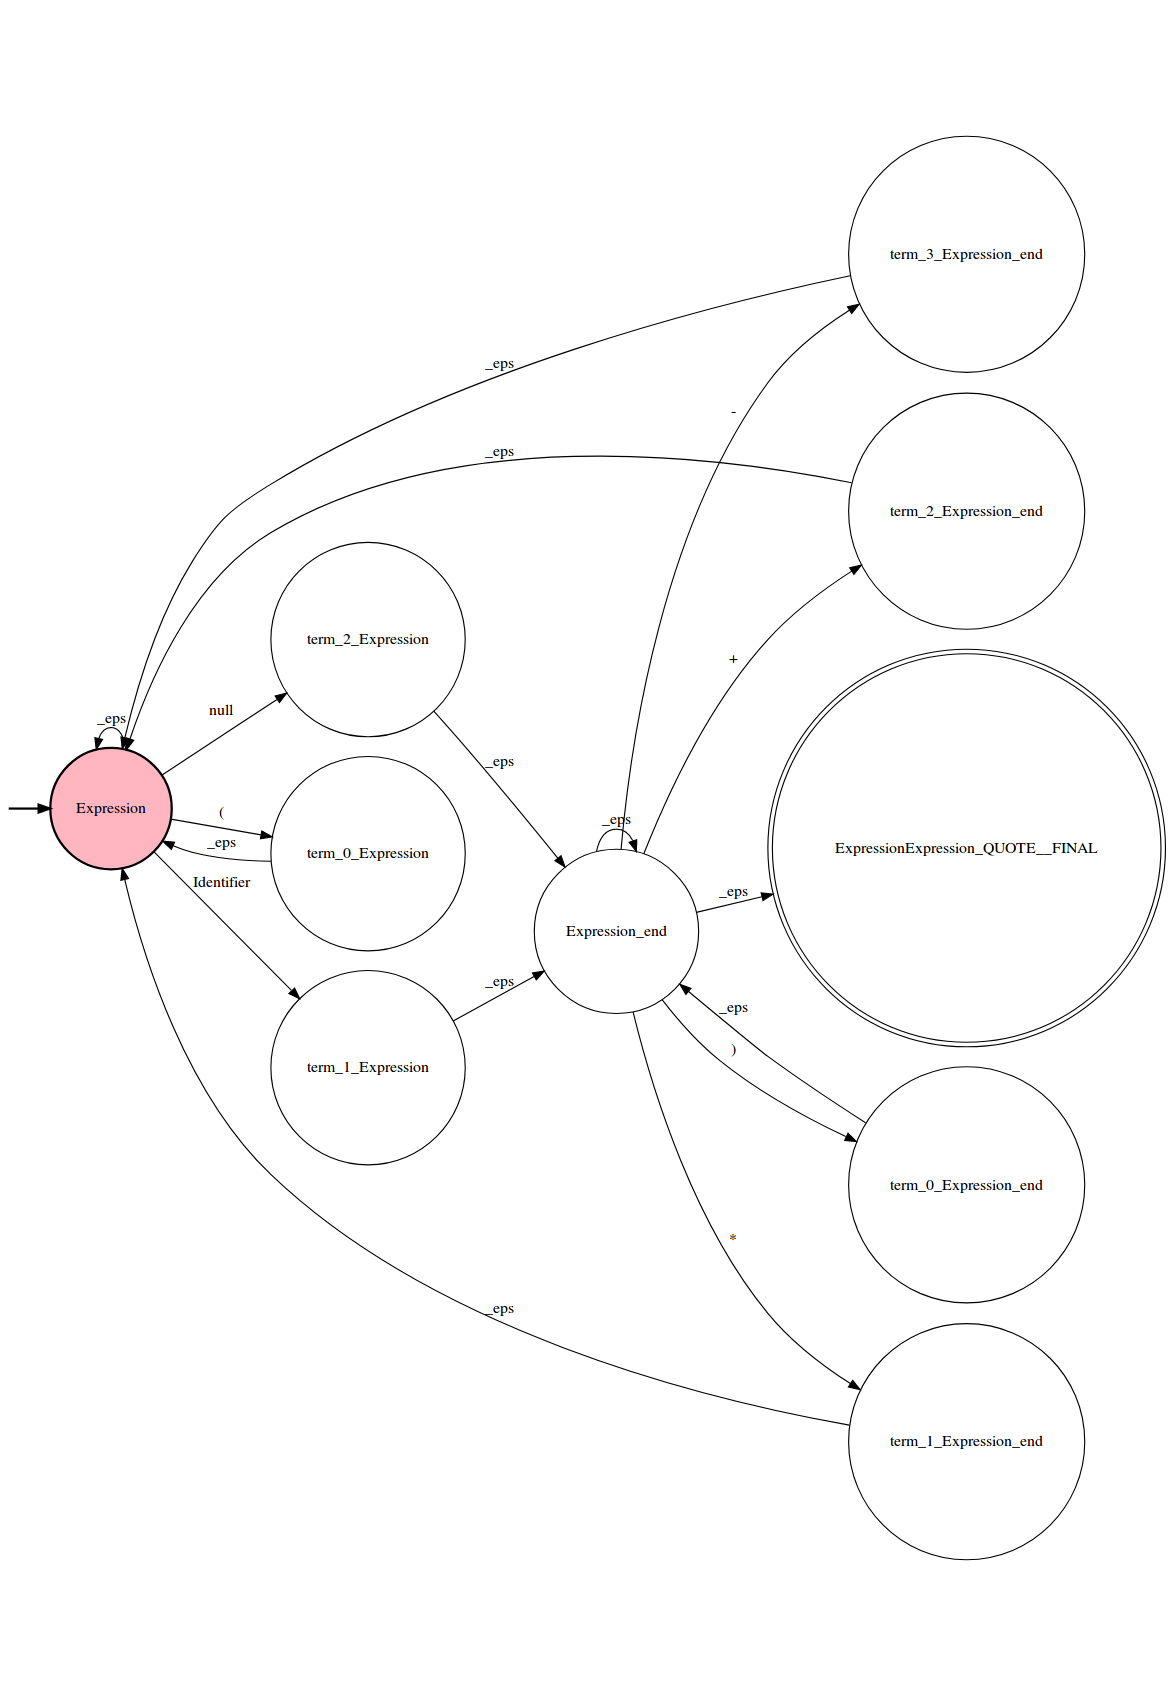
\includegraphics[scale=0.35]{Figures/advancedGrammar_NFA.png}
	\decoRule
 	\caption[NFA for Expression]{The NFA for Expression, produced from the strongly regular approximation}
 	\label{fig:advancedGrammar:NFA:Expression}
\end{figure}


\pagebreak\subsection{DFA for strongly regular Expression}
\begin{figure}[h]
	\centering
	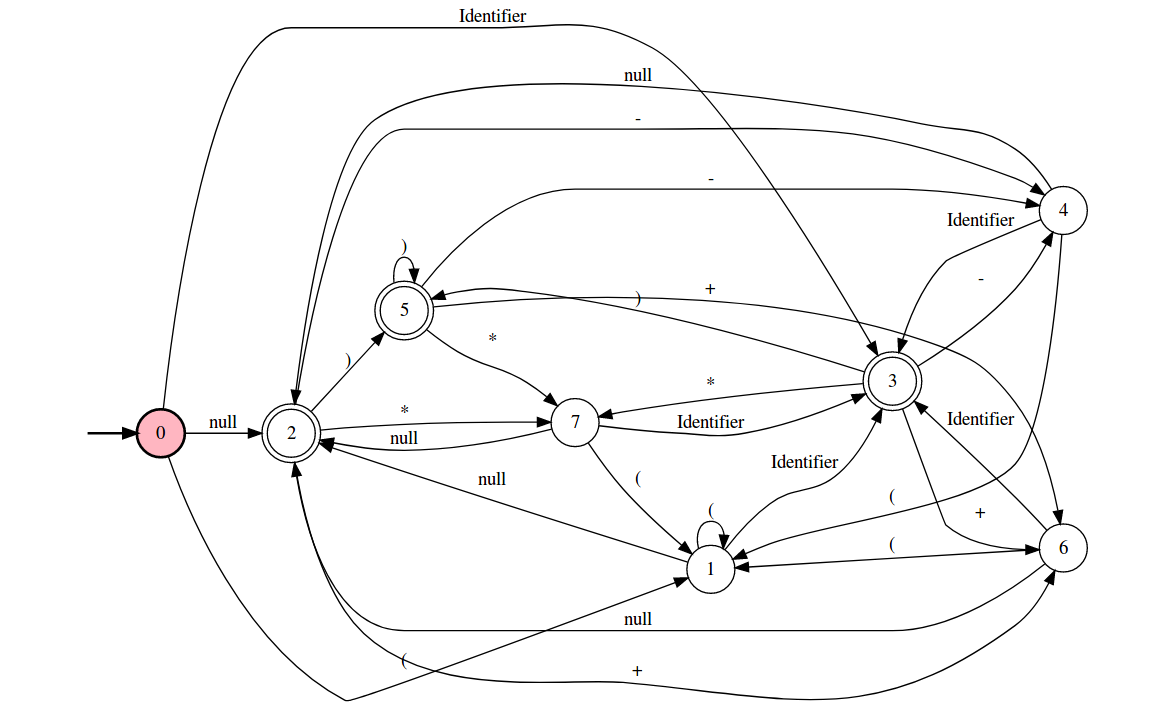
\includegraphics[scale=0.42]{Figures/advancedGrammar_DFA.png}
	\decoRule
 	\caption[DFA for Expresion]{The DFA for Expression, produced from the strongly regular approximation}
 	\label{fig:advancedGrammar:DFA:Expression}
\end{figure}

